\documentclass[conference]{IEEEtran}
\IEEEoverridecommandlockouts

\usepackage{amsmath,amssymb}
\usepackage{graphicx}
\usepackage{booktabs}
\usepackage{tikz}
\usetikzlibrary{arrows.meta, positioning}
\usepackage{cite}
\usepackage{url}

\begin{document}

\title{Sketch-to-Face Synthesis Using a Conditional Generative Adversarial Network}

\author{
\IEEEauthorblockN{Hassan Younas}
\IEEEauthorblockA{Roll No: 21I-1788 \\
Department of Computer Science \\
Generative AI -- Assignment 2, Question 3}
}

\maketitle

\begin{abstract}
This report presents a conditional generative adversarial network (cGAN) that translates
hand-drawn face sketches into photorealistic face images. Following the image-to-image
translation formulation of Isola \textit{et al.} (pix2pix), the model pairs a U-Net
encoder-decoder generator with a conditional PatchGAN discriminator, trained on the
Person Face Sketches dataset with an adversarial loss combined with a weighted
$L_1$ reconstruction loss. The model was trained for 100 epochs on a subsampled
6{,}000-pair training set under a fixed Kaggle GPU compute budget, using mixed-precision
training to keep the run within a single session. We report quantitative
($L_1 = 0.3035$, PSNR $= 13.30$\,dB) and qualitative results, and analyze the specific
factors -- dataset subsampling, the ill-posed nature of sketch-to-photo mapping, and the
adversarial loss objective itself -- that explain the observed result quality.
\end{abstract}

\begin{IEEEkeywords}
conditional GAN, image-to-image translation, pix2pix, U-Net, PatchGAN, face synthesis
\end{IEEEkeywords}

\section{Introduction}

Generative Adversarial Networks (GANs) \cite{goodfellow2014gan} learn to produce data
that is indistinguishable from a real data distribution by pitting a generator against a
discriminator in a minimax game. The original formulation offers no control over what the
generator produces; Mirza and Osindero's Conditional GAN (cGAN) \cite{mirza2014cgan}
addresses this by conditioning both networks on auxiliary information -- commonly a class
label. This work uses a full \emph{image} as the conditioning signal rather than a label,
which is the setting formalized by Isola \textit{et al.} as ``image-to-image translation''
(pix2pix) \cite{isola2017pix2pix}. The specific task addressed here is sketch-to-face
synthesis: given a hand-drawn or edge-extracted sketch of a face, generate the
corresponding realistic photograph.

The remainder of this report describes the dataset and preprocessing pipeline
(Section~\ref{sec:methodology}), the generator/discriminator architecture and training
procedure, the quantitative and qualitative results obtained
(Section~\ref{sec:results}), and an analysis of the specific factors that produced these
results (Section~\ref{sec:discussion}).

\section{Methodology}
\label{sec:methodology}

\subsection{Dataset}

The model was trained on the \emph{Person Face Sketches} dataset \cite{sketchdataset},
which provides paired sketch/photo images with a predefined train/validation split. Pairs
were located and matched by filename stem within each split's \texttt{sketches/} and
\texttt{photos/} subdirectories, using the immediate parent directory name to classify
each file's domain (rather than the full file path, since the dataset's root directory
name itself contains the substring ``sketch'' and would otherwise misclassify every
file). To keep total training time within a single Kaggle GPU session, the training and
validation sets were randomly subsampled to 6{,}000 and 1{,}000 pairs respectively (from
the dataset's considerably larger predefined splits), with a fixed random seed for
reproducibility.

\subsection{Preprocessing and Augmentation}

Each sketch/photo pair was resized to $286\times286$ and then jointly random-cropped to
$256\times256$, with an identical random horizontal flip applied to both images of a
pair, so spatial alignment between sketch and target photo is preserved under
augmentation. Validation pairs use a deterministic center crop instead. All images were
normalized to $[-1,1]$ per channel to match the generator's $\tanh$ output range.

\subsection{Network Architecture}

\textbf{Generator.} The generator is a U-Net \cite{ronneberger2015unet} with 8
stride-2 convolutional downsampling blocks and 7 corresponding transposed-convolution
upsampling blocks plus a final output layer, illustrated in
Fig.~\ref{fig:generator}. Skip connections concatenate each encoder block's feature map
with the decoder block at the matching spatial resolution, allowing fine spatial detail
present in the input sketch (edges, facial proportions) to bypass the bottleneck
entirely rather than being reconstructed from a heavily compressed
$1\times1$ representation. Downsampling blocks use Conv-InstanceNorm-LeakyReLU
($\alpha=0.2$); upsampling blocks use ConvTranspose-InstanceNorm-ReLU, with dropout
($p=0.5$) applied to the innermost layers as a stochastic regularizer. The final layer
uses $\tanh$ to map to the $[-1,1]$ output range.

\begin{figure*}[t]
\centering
\resizebox{\textwidth}{!}{%
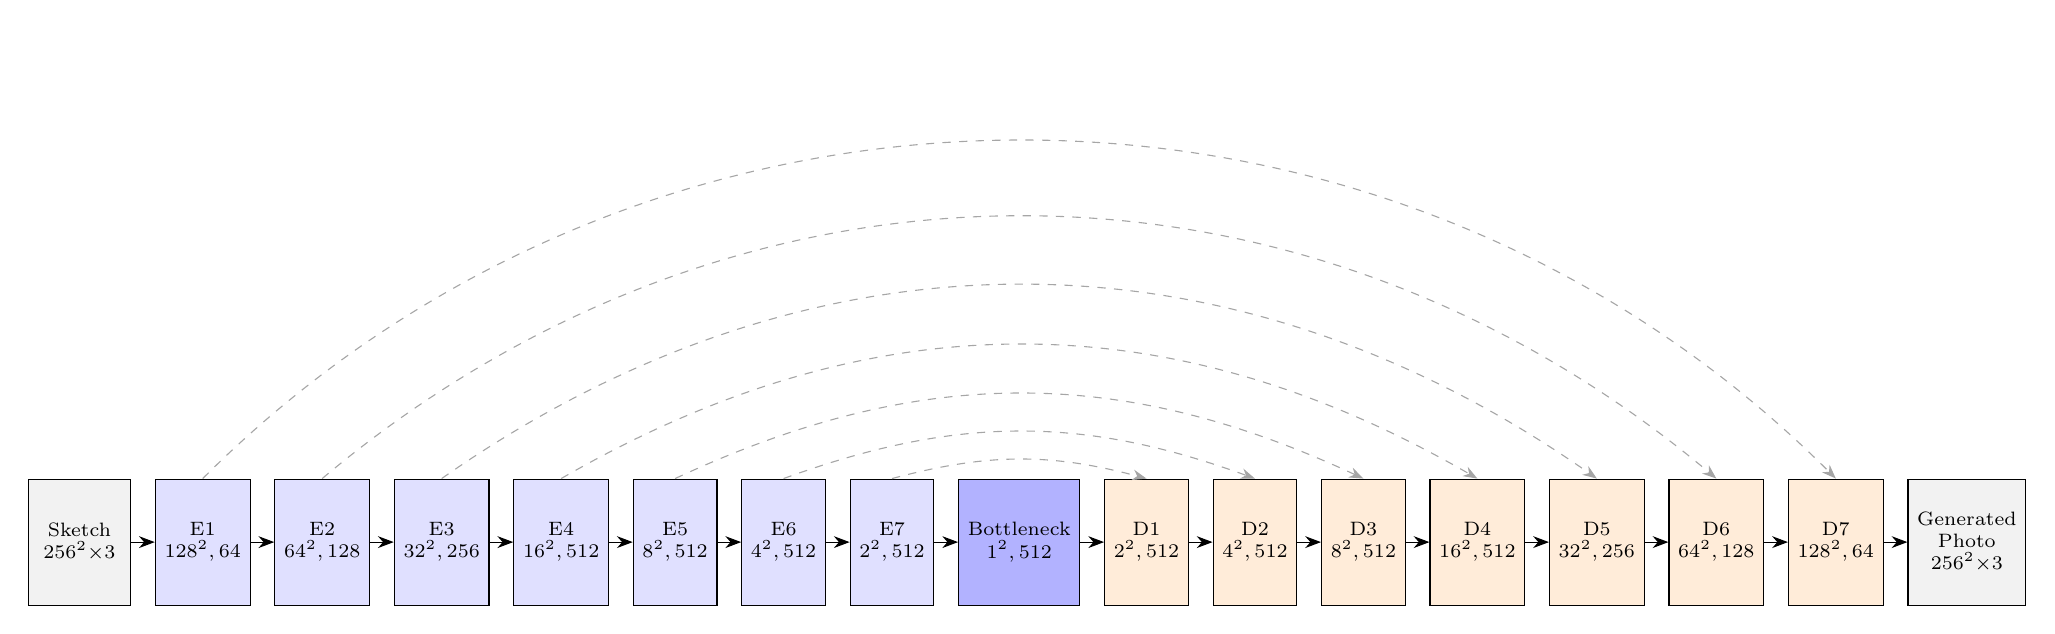
\begin{tikzpicture}[
  font=\scriptsize,
  enc/.style={draw, fill=blue!12, minimum width=0.9cm, minimum height=1.6cm, align=center},
  dec/.style={draw, fill=orange!15, minimum width=0.9cm, minimum height=1.6cm, align=center},
  io/.style={draw, fill=gray!10, minimum width=1.3cm, minimum height=1.6cm, align=center},
  arr/.style={-{Stealth[length=2mm]}},
  skip/.style={-{Stealth[length=1.8mm]}, dashed, gray!70}
]
\node[io] (sk) {Sketch\\$256^2{\times}3$};
\node[enc, right=0.3cm of sk]  (e1) {E1\\$128^2,64$};
\node[enc, right=0.3cm of e1]  (e2) {E2\\$64^2,128$};
\node[enc, right=0.3cm of e2]  (e3) {E3\\$32^2,256$};
\node[enc, right=0.3cm of e3]  (e4) {E4\\$16^2,512$};
\node[enc, right=0.3cm of e4]  (e5) {E5\\$8^2,512$};
\node[enc, right=0.3cm of e5]  (e6) {E6\\$4^2,512$};
\node[enc, right=0.3cm of e6]  (e7) {E7\\$2^2,512$};
\node[enc, right=0.3cm of e7, fill=blue!30]  (e8) {Bottleneck\\$1^2,512$};

\node[dec, right=0.3cm of e8]  (d7) {D1\\$2^2,512$};
\node[dec, right=0.3cm of d7]  (d6) {D2\\$4^2,512$};
\node[dec, right=0.3cm of d6]  (d5) {D3\\$8^2,512$};
\node[dec, right=0.3cm of d5]  (d4) {D4\\$16^2,512$};
\node[dec, right=0.3cm of d4]  (d3) {D5\\$32^2,256$};
\node[dec, right=0.3cm of d3]  (d2) {D6\\$64^2,128$};
\node[dec, right=0.3cm of d2]  (d1) {D7\\$128^2,64$};
\node[io, right=0.3cm of d1]   (out) {Generated\\Photo\\$256^2{\times}3$};

\draw[arr] (sk) -- (e1);
\draw[arr] (e1) -- (e2);
\draw[arr] (e2) -- (e3);
\draw[arr] (e3) -- (e4);
\draw[arr] (e4) -- (e5);
\draw[arr] (e5) -- (e6);
\draw[arr] (e6) -- (e7);
\draw[arr] (e7) -- (e8);
\draw[arr] (e8) -- (d7);
\draw[arr] (d7) -- (d6);
\draw[arr] (d6) -- (d5);
\draw[arr] (d5) -- (d4);
\draw[arr] (d4) -- (d3);
\draw[arr] (d3) -- (d2);
\draw[arr] (d2) -- (d1);
\draw[arr] (d1) -- (out);

\draw[skip] (e1.north) to[bend left=45] (d1.north);
\draw[skip] (e2.north) to[bend left=40] (d2.north);
\draw[skip] (e3.north) to[bend left=35] (d3.north);
\draw[skip] (e4.north) to[bend left=30] (d4.north);
\draw[skip] (e5.north) to[bend left=25] (d5.north);
\draw[skip] (e6.north) to[bend left=20] (d6.north);
\draw[skip] (e7.north) to[bend left=15] (d7.north);
\end{tikzpicture}}
\caption{U-Net generator: 8 stride-2 encoder blocks (blue) mirrored by 7 decoder blocks
(orange) plus a final output layer, with skip connections (dashed arcs) concatenating
same-resolution encoder/decoder feature maps. Labels show output spatial resolution and
channel count at each stage.}
\label{fig:generator}
\end{figure*}

\textbf{Discriminator.} The discriminator (Fig.~\ref{fig:discriminator}) is a conditional
PatchGAN. The sketch and a candidate photo (either the real target or the generator's
output) are concatenated channel-wise into a 6-channel input and passed through four
convolutional blocks, producing a $30\times30$ grid of real/fake scores rather than a
single scalar. Each output unit's receptive field corresponds to a $70\times70$ patch of
the input, so the discriminator penalizes local texture realism rather than judging the
image as a whole -- this was the deliberate design choice made by Isola \textit{et al.}
to encourage sharp, locally-realistic output while keeping the discriminator's task
tractable and its gradient signal stable throughout training.

\begin{figure}[t]
\centering
\resizebox{\linewidth}{!}{%
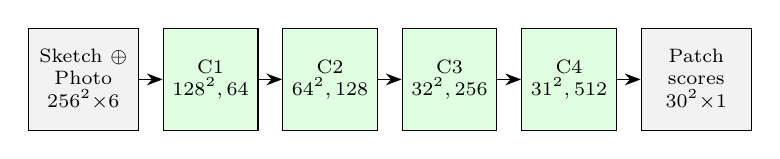
\begin{tikzpicture}[
  font=\scriptsize,
  cblock/.style={draw, fill=green!12, minimum width=1.0cm, minimum height=1.3cm, align=center},
  io/.style={draw, fill=gray!10, minimum width=1.4cm, minimum height=1.3cm, align=center},
  arr/.style={-{Stealth[length=2mm]}}
]
\node[io] (in) {Sketch $\oplus$\\Photo\\$256^2{\times}6$};
\node[cblock, right=0.3cm of in] (c1) {C1\\$128^2,64$};
\node[cblock, right=0.3cm of c1] (c2) {C2\\$64^2,128$};
\node[cblock, right=0.3cm of c2] (c3) {C3\\$32^2,256$};
\node[cblock, right=0.3cm of c3] (c4) {C4\\$31^2,512$};
\node[io, right=0.3cm of c4] (out) {Patch\\scores\\$30^2{\times}1$};

\draw[arr] (in) -- (c1);
\draw[arr] (c1) -- (c2);
\draw[arr] (c2) -- (c3);
\draw[arr] (c3) -- (c4);
\draw[arr] (c4) -- (out);
\end{tikzpicture}}
\caption{Conditional PatchGAN discriminator. The sketch and a candidate photo are
concatenated channel-wise and classified as real/fake at the level of overlapping
$70\times70$ patches rather than the whole image.}
\label{fig:discriminator}
\end{figure}

\subsection{Loss Function and Training Details}

Following pix2pix, the generator is trained with a combined objective:
\begin{equation}
\mathcal{L}_G = \mathcal{L}_{\text{GAN}}(G,D) + \lambda \, \mathcal{L}_{L_1}(G),
\qquad \lambda = 100,
\label{eq:loss}
\end{equation}
where $\mathcal{L}_{\text{GAN}}$ is a binary cross-entropy adversarial loss and
$\mathcal{L}_{L_1}$ is the mean absolute pixel-wise error between the generated and
target photo. The large weighting on $\mathcal{L}_{L_1}$ anchors the generator's output
to the ground-truth structure, while the adversarial term supplies high-frequency
realism that $L_1$ alone tends to blur out. The discriminator is trained to maximize its
ability to separate real $(sketch, photo)$ pairs from generated
$(sketch, G(sketch))$ pairs, using the standard binary cross-entropy GAN loss.

Both networks were optimized with Adam ($\text{lr}=2\times10^{-4}$, $\beta_1=0.5$,
$\beta_2=0.999$), the low-momentum $\beta_1$ being a standard stabilization choice for
adversarial training. Training ran for 100 epochs with batch size 32, under automatic
mixed precision (AMP) and cuDNN kernel autotuning, on a single Kaggle GPU session. A
full checkpoint (both networks, both optimizers, and AMP scaler state) was written
atomically after every epoch to allow seamless resumption after a session interruption.

\section{Results}
\label{sec:results}

\subsection{Training Dynamics}

Fig.~\ref{fig:loss} shows the generator and discriminator loss over all 100 epochs.
$\mathcal{L}_G$ decreased smoothly and monotonically from 42.52 to 31.58, visibly
plateauing after approximately epoch 60--70 (minimum value 31.27, reached at epoch 93,
statistically indistinguishable from the final epoch's 31.58). $\mathcal{L}_D$ remained
stable throughout, oscillating within a $0.22$--$0.45$ band with no divergence or
collapse toward zero. Average epoch time was 67.0\,s, giving a total training time of
111.7 minutes ($\approx$1.86 hours).

\begin{figure}[t]
\centering
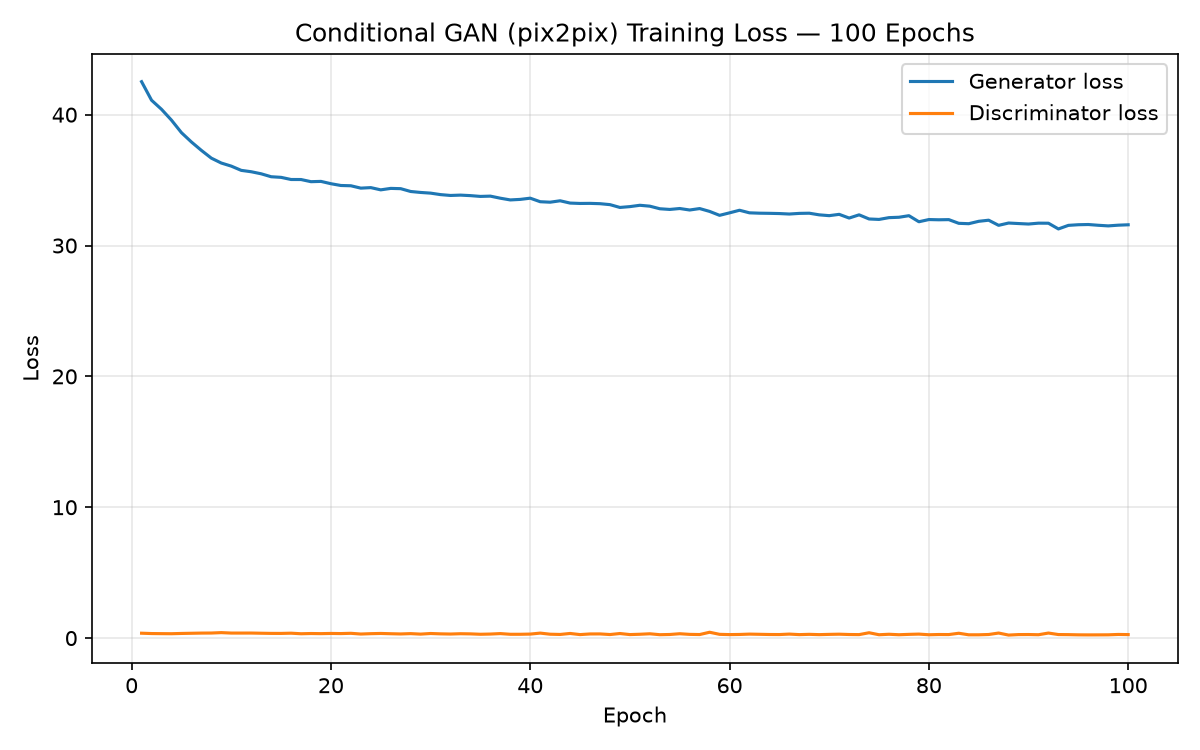
\includegraphics[width=\linewidth]{loss_curve.png}
\caption{Generator and discriminator training loss over 100 epochs. The generator loss
is dominated by the $\lambda=100$ weighted $L_1$ term and plateaus after
epoch $\approx$60--70; the discriminator loss remains stable, indicating balanced
adversarial training with no mode collapse.}
\label{fig:loss}
\end{figure}

\subsection{Quantitative Results}

Table~\ref{tab:results} summarizes the final training losses and validation-set metrics.
Validation $L_1$ (measured directly on $[-1,1]$-normalized pixel values, independent of
the $\lambda=100$ training weight) was 0.3035, and PSNR was 13.30\,dB.

\begin{table}[t]
\centering
\caption{Summary of Training and Validation Results}
\label{tab:results}
\begin{tabular}{@{}ll@{}}
\toprule
Metric & Value \\
\midrule
Training pairs (subsampled) & 6{,}000 \\
Validation pairs (subsampled) & 1{,}000 \\
Epochs & 100 \\
Final generator loss ($\mathcal{L}_G$) & 31.58 \\
Final discriminator loss ($\mathcal{L}_D$) & 0.266 \\
Minimum generator loss (epoch) & 31.27 (epoch 93) \\
Average epoch time & 67.0 s \\
Total training time & 111.7 min ($\approx$1.86 h) \\
Validation $L_1$ ($[-1,1]$ scale) & 0.3035 \\
Validation PSNR & 13.30 dB \\
\bottomrule
\end{tabular}
\end{table}

\subsection{Qualitative Results}

Fig.~\ref{fig:progression} compares sample outputs from an early training epoch against
a later, converged epoch, each showing the input sketch (top row), generated photo
(middle row), and ground-truth photo (bottom row) for four validation examples. Early in
training, outputs show a pronounced regular grid/checkerboard pattern overlaid on an
otherwise blurred, low-detail face -- a well-documented artifact of randomly-initialized
transposed-convolution upsampling layers \cite{odena2016checkerboard}. By the later
epoch, this artifact has been almost entirely learned away: outputs show coherent facial
structure, hair color and style consistent with the sketch, plausible skin tone, and
expression matching the input, though with some softness and localized texture
artifacts (e.g., around the mouth) remaining.

\begin{figure}[t]
\centering
% TODO: replace with the actual files from samples/, e.g. epoch_001.png and epoch_100.png
\includegraphics[width=\linewidth]{sample_epoch_early.png}
\\[2pt]
\includegraphics[width=\linewidth]{sample_epoch_late.png}
\caption{Qualitative progression over training. Each triptych shows sketch (top),
generated photo (middle), and ground-truth photo (bottom) for four validation samples.
\textbf{Top block:} an early training epoch, showing characteristic checkerboard
artifacts from an undertrained decoder. \textbf{Bottom block:} a later, converged
epoch, showing substantially improved structural and textural fidelity.}
\label{fig:progression}
\end{figure}

\section{Discussion: Analysis of Results}
\label{sec:discussion}

This section analyzes \emph{why} the model produced the specific results reported above,
rather than restating them.

\textbf{The generator loss is directly explained by the measured $L_1$ error.} With
$\lambda=100$ in Eq.~\ref{eq:loss}, the $L_1$ term alone should contribute
approximately $100 \times 0.3035 \approx 30.4$ to the final generator loss; the observed
final loss of 31.58 leaves only $\approx$1.2 attributable to the adversarial term. This
confirms the loss is behaving exactly as designed: $L_1$ dominates and anchors the
output, while the adversarial component contributes a comparatively small but
consistent correction pushing toward realism. This also explains why $\mathcal{L}_G$
plateaus once $L_1$ stops improving -- with a fixed, subsampled 6{,}000-pair training
set and a fully-capacity U-Net (no channel reduction was applied), the network reaches
the limit of what that data volume can teach it well before epoch 100.

\textbf{The modest PSNR (13.30\,dB) reflects the ill-posed nature of the task, not
primarily a training failure.} A sketch specifies edges and coarse facial structure but
leaves skin tone, exact hair color and texture, lighting, and background completely
unconstrained -- many different photographs are equally valid completions of the same
sketch. A GAN trained with an adversarial loss is explicitly optimized to produce
\emph{a} plausible photograph, not to reconstruct \emph{the specific} ground-truth pixel
values, so it will systematically incur pixel-wise error even when its output looks
convincing. This is the same limitation Isola \textit{et al.} note in the original
pix2pix work: $L_1$/PSNR-style metrics correlate poorly with perceptual quality for
adversarially-trained image translation, precisely because the objective they are
trained under does not optimize for pixel alignment. The qualitative results in
Fig.~\ref{fig:progression} should therefore be weighted more heavily than
Table~\ref{tab:results}'s PSNR figure when judging output quality.

\textbf{Dataset subsampling is a second, compounding factor.} Training used 6{,}000 of
the dataset's considerably larger available pairs, chosen specifically to fit training
within a single Kaggle GPU session. A smaller, less diverse training set gives the
generator less exposure to the range of skin tones, hairstyles, and facial structures
present in the validation set, which directly increases pixel-level validation error even
where the qualitative structure is captured correctly.

\textbf{The discriminator loss staying stable in the 0.22--0.45 range, never collapsing
toward 0 or diverging toward saturation, indicates healthy adversarial dynamics.} This
stability is attributable to two specific design choices: the PatchGAN's patch-level
classification task is inherently easier and lower-variance for the discriminator than
whole-image classification, which keeps its gradient signal to the generator informative
throughout training rather than saturating early; and the Adam $\beta_1=0.5$ setting
reduces the momentum-driven oscillation that commonly destabilizes adversarial training
at the default $\beta_1=0.9$. Neither network overpowered the other at any point in the
100 epochs, which is direct evidence against mode collapse.

\textbf{The checkerboard artifact visible in early-epoch outputs (Fig.~\ref{fig:progression},
top) is a documented, expected property of transposed convolutions, not a bug.}
ConvTranspose2d layers with overlapping kernel strides produce uneven overlap in their
output feature maps at initialization, before training has had a chance to learn weights
that compensate for the resulting grid pattern \cite{odena2016checkerboard}. That this
pattern is visibly reduced by the later epoch (Fig.~\ref{fig:progression}, bottom)
is itself evidence that training converged correctly rather than stalling.

\section{Limitations and Future Work}

The reported results reflect a compute-constrained training budget: 6{,}000 of the
available training pairs, 100 epochs, and full model capacity (channel widths were kept
at pix2pix's original settings rather than reduced). Restoring the full training set,
increasing training duration beyond the plateau observed near epoch 70, or increasing
$\lambda$ selectively would each be expected to reduce validation $L_1$/PSNR further,
though based on the discussion above, perceptual quality gains are likely to
saturate faster than pixel-wise metrics suggest. A perceptual metric such as LPIPS or
FID, which better correlates with human judgment of GAN output quality than $L_1$/PSNR,
would be a valuable addition to future evaluation.

\section{Conclusion}

A pix2pix-style conditional GAN, comprising a U-Net generator and a conditional
PatchGAN discriminator, was trained to translate face sketches into photorealistic
images. Training was stable across 100 epochs with no evidence of mode collapse, and
qualitative results show a clear, explicable improvement from early, checkerboard-artifacted
outputs to structurally coherent, texture-consistent generated faces by later epochs.
The modest quantitative $L_1$/PSNR scores are shown to be substantially attributable to
the inherent ill-posedness of sketch-to-photo translation and the dataset subsampling
used to fit training within a single GPU session, rather than to a failure of the
training procedure itself.

\section*{Prompts}

The following is a condensed log of the prompts used to develop this project with an AI
coding assistant (Claude), grouped by development stage.

\begin{enumerate}
\item \textit{Initial implementation:} ``I want you to read and understand this
assignment's Question 3 carefully and implement it.''
\item \textit{Debugging dataset pairing (0 pairs found):} shared the notebook error
output and asked for a fix; iterated again after a second failure caused by the dataset
root directory name itself containing the substring ``sketch''.
\item \textit{Environment troubleshooting:} shared a Kaggle \texttt{pip install} network
error and asked for a fix; asked whether the assistant could access the Kaggle notebook
URL directly (it could not, and explained why).
\item \textit{Verification:} ``i guess i messed up the code again, can you please check
if code is not altered and correct?''
\item \textit{Performance estimation:} ``how much time it should take for 1 epoch on
kaggle GPU?'' followed by a request to add per-epoch timing and mixed-precision (AMP)
support, and to explain the ETA calculation.
\item \textit{Reliability fix:} shared a disk-write \texttt{RuntimeError} during
checkpoint saving; requested and received a fix bounding checkpoint disk usage and
making checkpoint writes atomic.
\item \textit{Speed optimization:} ``it's taking too long to run, do you have any other
alternate solution?'' -- selected dataset subsampling and free/no-quality-cost
optimizations (cuDNN autotuning, larger batch size, more data workers) from the options
presented.
\item \textit{API deprecation fix:} shared a \texttt{torch.cuda.amp} \texttt{FutureWarning}
and requested migration to the current \texttt{torch.amp} API.
\item \textit{Post-training workflow:} ``now i've run all the cells. what should i do
next?'' followed by requests for a results-bundling script and a one-click download link
for Kaggle.
\item \textit{Results analysis and report generation:} shared the trained model's loss
history, run summary, sample output grids, and validation $L_1$/PSNR, and requested this
LaTeX report including an architecture diagram and an analysis of the reasons behind the
observed results.
\end{enumerate}

\begin{thebibliography}{00}
\bibitem{goodfellow2014gan} I. Goodfellow, J. Pouget-Abadie, M. Mirza, B. Xu, D. Warde-Farley,
S. Ozair, A. Courville, and Y. Bengio, ``Generative Adversarial Networks,'' in
\textit{Advances in Neural Information Processing Systems (NeurIPS)}, 2014.

\bibitem{mirza2014cgan} M. Mirza and S. Osindero, ``Conditional Generative Adversarial
Nets,'' \textit{arXiv preprint arXiv:1411.1784}, 2014.

\bibitem{isola2017pix2pix} P. Isola, J.-Y. Zhu, T. Zhou, and A. A. Efros, ``Image-to-Image
Translation with Conditional Adversarial Networks,'' in \textit{Proc. IEEE Conference on
Computer Vision and Pattern Recognition (CVPR)}, 2017.

\bibitem{ronneberger2015unet} O. Ronneberger, P. Fischer, and T. Brox, ``U-Net:
Convolutional Networks for Biomedical Image Segmentation,'' in \textit{Medical Image
Computing and Computer-Assisted Intervention (MICCAI)}, 2015.

\bibitem{odena2016checkerboard} A. Odena, V. Dumoulin, and C. Olah, ``Deconvolution and
Checkerboard Artifacts,'' \textit{Distill}, 2016.

\bibitem{sketchdataset} ``Person Face Sketches,'' Kaggle dataset,
\url{https://www.kaggle.com/datasets/almightyj/person-face-sketches}.

\end{thebibliography}

\end{document}
